\section{Full capped-budget grid}
\label{app:capped}

\begin{table}[H]
\centering
\small
\tablecapped
\caption{Mean episode-restricted recall accuracy (three seeds) by arm, KV
budget, and evaluation context length on the primary cell. The matrix
fast-weight model's state is 32{,}768 bytes at every entry of its row; the
transformer's cap at budget $M$ pins its total KV bytes across layers and
heads to $M \times 32{,}768$. $M{=}1$ is excluded from the registered walk
because its cap length (8 tokens) sits below the query length; its
descriptive readings, 0.021 to 0.030 across seeds and horizons, sit at
chance like every other transformer entry. Chance is 0.031; the
demonstration bar is 0.094; no transformer entry approaches
either.} % <!-- evidence: C4 -->
\label{tab:capped}
\end{table}

\section{Linear read-out sites}
\label{app:taps}

\begin{table}[H]
\centering
\small
\tabletaps
\caption{Offline ridge-probe recovery of the bound value's target vector
by read-out site, on the single-seed localization checkpoints (fit on
24{,}576 fresh draws, evaluated on the pinned 4{,}096-query set;
``rf@0.9'' is the fraction of queries whose predicted vector clears cosine
0.9 against the target; ``gap'' is cosine mean minus a shuffled-fit
control). No linear combine of a raw recurrent state and the query clears
the threshold in either arm, including the read placed directly on the
causally necessary $S_0$; only the pre-LM-head hidden state decodes, and
only in the matrix fast-weight arm.} % <!-- evidence: C6 -->
\label{tab:taps}
\end{table}

\section{Training-loss trajectories, all three arms}
\label{app:traincurve}

\begin{figure}[H]
\centering
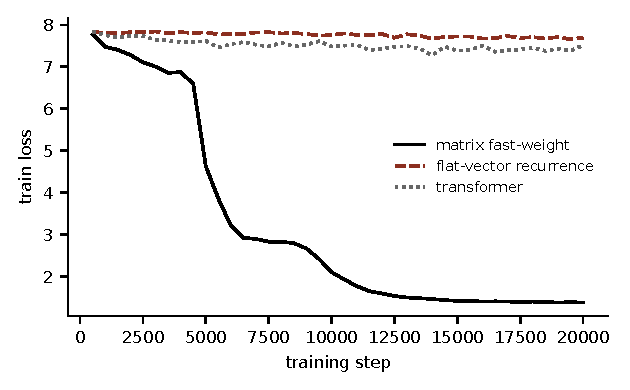
\includegraphics[width=0.62\linewidth]{figures/fig3_traincurve.pdf}
\caption{Training loss (primary task, seed 0) over the full
20{,}000-step run, all three arms, from the same archived configs used
for the parameter counts in Section~\ref{sec:setup}. The flat-vector and
transformer arms drop to 7.83 and 7.84 by step 500 and move only to 7.69
and 7.51 over the remaining 19{,}500 steps; the matrix fast-weight arm
keeps falling for the entire run, reaching
1.38. % <!-- evidence: C11 -->
Learning rate ($3\times10^{-4}$), warmup, and auxiliary-loss weighting
were shared across the three architecturally distinct mixers and were not
independently tuned per arm; a per-architecture learning-rate sensitivity
sweep was not run. The claim in Section~\ref{sec:recall} is scoped to
this shared training budget accordingly.}
\label{fig:traincurve}
\end{figure}

\section{Reproducibility of every number}
\label{app:repro}

Every figure and every table cell in this paper regenerates from archived
evaluation artifacts by a single versioned script that asserts the MD5
checksum of each source file before loading it; a changed artifact fails
the build rather than silently changing a number. Every inline numerical
claim in the source carries a machine-checkable comment naming its row in
a claims-to-evidence map maintained alongside the draft. The archived
artifacts, the script, and the map will be released with the
de-anonymized version of this paper.
